

\thispagestyle{empty}
\colorlet{shadecolor}{\chapterColor}
\chapter{Quartzville Creek}

\fancyhead{}
\lhead[\textcolor{\chapterColor}{\rule[-2pt]{\textwidth}{15pt}}]{\textcolor{\chapterColor}{\rule[-2pt]{\textwidth}{15pt}}\hspace{-\textwidth}\color{white}\hspace{4pt}\protect\thepage\hspace{1ex}-\hspace{1ex}Quartzville Creek}
\rhead[\textcolor{\chapterColor}{\rule[-2pt]{\textwidth}{15pt}}\hspace{-\textwidth}\color{white}Quartzville Creek \protect\thepage \hspace{4pt}]{\textcolor{\chapterColor}{\rule[-2pt]{\textwidth}{15pt}}}
\fancyhead[RO]{}
\fancyhead[RE]{\color{white}Quartzville Creek\hspace{1ex}-\hspace{1ex}\protect\thepage \hspace{4pt}}


\raggedcolumns
\begin{multicols}{2}

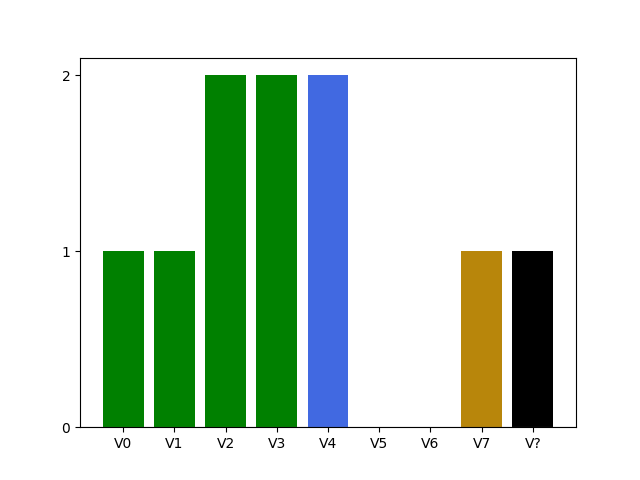
\includegraphics[width=\linewidth]{./maps/plots//Quartzville Creek.png}
\end{multicols}
\begin{multicols}{2}

About an hour further down the road from the main area there are a few interesting boulders in a creek. Generally lower temperatures, free camping, and pleasant swimming holes make this a nice mid summer spot.\\



\null\newpage
\phantomsection\label{sm:Redneck Riviera area map}
	\setbox0=\hbox{\begin{overpic}[width=0.8\linewidth]{./maps/area/out/redneck_c.png}
	\end{overpic}}
	\needspace{\ht0}
	\begin{center}
	\begin{overpic}[width=0.9\linewidth]{./maps/area/out/redneck_c.png}
	\end{overpic}
	\end{center}


\section{A - Redneck Riviera}\phantomsection\label{sa:Redneck Riviera}
\setbox0=\hbox{
\includegraphics[width=0.45\linewidth]{./maps/qr//Redneck Riviera_qr.png}}% Store image in \box0
\needspace{\ht0}% Need at least the height of \box0
\begin{center}

\includegraphics[width=0.45\linewidth]{./maps/qr//Redneck Riviera_qr.png}
\end{center}
\begin{center}
\underline{\textcolor{blue}{\href{http://maps.google.com/maps?q=44.570410945356336,-122.4060701729652}{Navigate to this sub area}}}
\end{center}


Redneck riviera is located on Quartzville road approximately 20.6 miles from highway 20 park in the gravel pull out on the creek side of the road. This is a nice spot with good swimming access and a few established routes on both sides of the river. The locals like to use this spot to pan for gold. Often they are friendly and willing to share the space.\\




\needspace{10em}
\subsection*{Pony Boy}\phantomsection\label{bf:Pony Boy}

A small boulder sits on the far bank of the river upriver from the parking.\\



\needspace{2em}
\phantomsection\label{rt:Pony Boy}
\colorbox{green!20}{
\parbox{0.95\linewidth}{
\hspace{-1ex}\textbf{$\Box$
1 Pony Boy V2 \ding{73} 
}}}
\begin{adjustwidth}{1.3em}{}			

Sit start with hands matched in a juggy pocket on the overhanging face of the boulder. Climbing this thing is probably not worth getting your pads wet.
  (No Topo)
\end{adjustwidth}




	\end{multicols}
\phantomsection\label{tp:Monorail}
	\setbox0=\hbox{\begin{overpic}[width=0.8\linewidth]{./maps/topos/Monorail_c.png}
	\end{overpic}}
	\needspace{\ht0}
	\begin{center}
	\begin{overpic}[width=0.9\linewidth]{./maps/topos/Monorail_c.png}
	\end{overpic}
	\end{center}

	\begin{multicols}{2}

\needspace{10em}
\subsection*{Monorail}\phantomsection\label{bf:Monorail}

Low boulder just below the parking area with an obvious sharp lip that spans the entire downhill face.\\



\needspace{2em}
\phantomsection\label{rt:Monorail}
\colorbox{Goldenrod!20}{
\parbox{0.95\linewidth}{
\hspace{-1ex}\textbf{$\Box$
2 Monorail V8+ \ding{72}\ding{72}\ding{72} 
}}}
\begin{adjustwidth}{1.3em}{}			

Start on the far right and traverse left along the lip. Topping in a shallow divot on the center left of the boulder.
\end{adjustwidth}


\begin{adjustwidth}{0.5cm}{}				
\needspace{4em}
\textbf{Variations:} \newline

\needspace{2em}
\phantomsection\label{vr:Monorail Extension Project}
\colorbox{red!20}{
\parbox{0.95\linewidth}{
\hspace{-1ex}\textbf{$\Box$
2a Mondorail V10 \ding{72}\ding{72}\ding{72} 
}}}
\begin{adjustwidth}{1.3em}{}			

Climb Monorail and ride the lip the whole way across the boulder.
\end{adjustwidth}



\end{adjustwidth}


\needspace{2em}
\phantomsection\label{rt:Deliverance}
\colorbox{Goldenrod!20}{
\parbox{0.95\linewidth}{
\hspace{-1ex}\textbf{$\Box$
3 Deliverance V7 \ding{72}\ding{72}\ding{72} 
}}}
\begin{adjustwidth}{1.3em}{}			

Sit start and climb the steep roof using a left hand side pull and the right facing rib. Top as for Monorail.
\end{adjustwidth}




\phantomsection\label{tp:Yo Mamma}
	\setbox0=\hbox{\begin{overpic}[width=0.8\linewidth]{./maps/topos/YoMamma_c.png}
	\end{overpic}}
	\needspace{\ht0}
	\begin{center}
	\begin{overpic}[width=0.9\linewidth]{./maps/topos/YoMamma_c.png}
	\end{overpic}
	\end{center}


\needspace{10em}
\subsection*{Yo Mamma Boulder}\phantomsection\label{bf:Yo Mamma Boulder}

Yo Mamma is bigger than any of the other boulders in this area. Look for it across the river and downstream from the parking.\\



\needspace{2em}
\phantomsection\label{rt:Ugly Face}
\colorbox{green!20}{
\parbox{0.95\linewidth}{
\hspace{-1ex}\textbf{$\Box$
4 Ugly Face V0 \ding{72} \warn
}}}
\begin{adjustwidth}{1.3em}{}			

Stand start on the left side of the west face of the boulder. This is also the down climb.
\end{adjustwidth}




\needspace{2em}
\phantomsection\label{rt:Binding of Isaac}
\colorbox{green!20}{
\parbox{0.95\linewidth}{
\hspace{-1ex}\textbf{$\Box$
5 Binding of Isaac V2 \ding{72}\ding{72} \warn
}}}
\begin{adjustwidth}{1.3em}{}			

Stand start with a left hand side pull about 5' left of Ugly face.
\end{adjustwidth}





\needspace{10em}
\subsection*{Moss Boss}\phantomsection\label{bf:Moss Boss}

A large mossy boulder on the roadside of the river and downstream of the parking area.\\



\needspace{2em}
\phantomsection\label{rt:Moss Boss}
\colorbox{green!20}{
\parbox{0.95\linewidth}{
\hspace{-1ex}\textbf{$\Box$
6 Moss Boss V3 \ding{72} 
}}}
\begin{adjustwidth}{1.3em}{}			

Believe it or not a route has been established and climbed on this dirty choss pile. Stand start on big holds on the river face and trend up and right finishing half way up the upstream face of the boulder. A direct finish is certainly possible too.
  (No Topo)
\end{adjustwidth}




	\end{multicols}
\phantomsection\label{tp:4.5}
	\setbox0=\hbox{\begin{overpic}[width=0.8\linewidth]{./maps/topos/45_c.png}
	\end{overpic}}
	\needspace{\ht0}
	\begin{center}
	\begin{overpic}[width=0.9\linewidth]{./maps/topos/45_c.png}
	\end{overpic}
	\end{center}

	\begin{multicols}{2}

\needspace{10em}
\subsection*{The 4.5}\phantomsection\label{bf:The 4.5}

Located on the river downstream and across the river from the parking. look for a clean "4.5° overhanging" face pointing downhill.\\



\needspace{2em}
\phantomsection\label{rt:Chicken Tendies}
\colorbox{green!20}{
\parbox{0.95\linewidth}{
\hspace{-1ex}\textbf{$\Box$
7 Chicken Tendies V1 \ding{72} 
}}}
\begin{adjustwidth}{1.3em}{}			

Stand start with hands matched on a good crimp rail on the left side of the boulder. Climb straight up.
\end{adjustwidth}




\needspace{2em}
\phantomsection\label{rt:Teenage Libertarians}
\colorbox{RoyalBlue!20}{
\parbox{0.95\linewidth}{
\hspace{-1ex}\textbf{$\Box$
8 Teenage Libertarians V4 \ding{72}\ding{72}\ding{72} 
}}}
\begin{adjustwidth}{1.3em}{}			

Start as for chicken tendies but traverse right and ascend the tallest part of the boulder.
\end{adjustwidth}




\needspace{2em}
\phantomsection\label{rt:Falcon's Reach}
\colorbox{green!20}{
\parbox{0.95\linewidth}{
\hspace{-1ex}\textbf{$\Box$
9 Falcon's Reach V3 \ding{72} 
}}}
\begin{adjustwidth}{1.3em}{}			

Squat start on a juggy edge. Climb straight up.
\end{adjustwidth}





\null\newpage

\section{B - Old Miner's Camp}\phantomsection\label{sa:Old Miner's Camp}
\setbox0=\hbox{
\includegraphics[width=0.45\linewidth]{./maps/qr//Old Miner's Camp_qr.png}}% Store image in \box0
\needspace{\ht0}% Need at least the height of \box0
\begin{center}

\includegraphics[width=0.45\linewidth]{./maps/qr//Old Miner's Camp_qr.png}
\end{center}
\begin{center}
\underline{\textcolor{blue}{\href{http://maps.google.com/maps?q=44.58651338802075,-122.35033857932665}{Navigate to this sub area}}}
\end{center}


Located on Quartzville approximately 24.8 miles from highway 20, the old miner's camp is a popular group campsite there are a few good sized boulders in the river. Only one boulder has established lines on it. Park either at the camp day use area or on the side of the road immediately above the Dab Rig boulder. Note: the dab rig boulder is typically underwater in the rainy season.\\



	\end{multicols}
\phantomsection\label{tp:Dab Rig}
	\setbox0=\hbox{\begin{overpic}[width=0.8\linewidth]{./maps/topos/DabRig_c.png}
	\end{overpic}}
	\needspace{\ht0}
	\begin{center}
	\begin{overpic}[width=0.9\linewidth]{./maps/topos/DabRig_c.png}
	\end{overpic}
	\end{center}

	\begin{multicols}{2}

\needspace{10em}
\subsection*{The Dab Rig}\phantomsection\label{bf:The Dab Rig}




\needspace{2em}
\phantomsection\label{rt:Unsalted Almonds}
\colorbox{Goldenrod!20}{
\parbox{0.95\linewidth}{
\hspace{-1ex}\textbf{$\Box$
1 Unsalted Almonds V8*  
}}}
\begin{adjustwidth}{1.3em}{}			

Sit start straddling the right arête with left hand on a diagonal edge and right hand on a sloper. Climb up and left across the well featured face.
\end{adjustwidth}




\needspace{2em}
\phantomsection\label{rt:Dank Commander}
\colorbox{RoyalBlue!20}{
\parbox{0.95\linewidth}{
\hspace{-1ex}\textbf{$\Box$
2 Dank Commander V4*  
}}}
\begin{adjustwidth}{1.3em}{}			

Start as for Unsalted Almonds, but go straight up.
\end{adjustwidth}






\end{multicols}
\clearpage